% !TeX program = xelatex
\documentclass[a4paper,10pt]{article}

% ============================================================================
% សន្លឹកកិច្ចការសិស្សបំពេញចន្លោះ ស-ខ្មៅ និងប្លង់ក្ដារខៀន/ចម្លើយគ្រូ (គ្មាន LCD / គ្មានកន្ត្រៃ)
% មេរៀនទី៥ (១.៤--១.៦)៖ ប្រមាណវិធីបូក ដក គុណ និងចែកឯកធា — ត្រូវគ្នានឹង LS_Plan_ALG52.tex
% ============================================================================
\usepackage[a4paper, left=1.0cm, right=1.0cm, top=0.75cm, bottom=1.00cm, footskip=0.52cm]{geometry}
\usepackage{amsmath}
\usepackage{unicode-math}
\usepackage{fontspec}
\usepackage{array, colortbl}
\usepackage[table]{xcolor}
\usepackage{enumitem}
\usepackage{pifont}
\usepackage{fancyhdr}
\usepackage{lastpage}
\usepackage{tikz}
\usepackage[most]{tcolorbox}
\usetikzlibrary{calc, arrows.meta, decorations.pathreplacing, positioning, babel}

\makeatletter
\let\@expl@@@mark@update@singlecol@structures@@\relax
\makeatother

\providecommand{\NGSFindFonts}{%
  \IfFileExists{C:/Windows/Fonts/cambria.ttc}{%
    \def\NGSSysPath{C:/Windows/Fonts/}%
    \def\NGSUserPath{C:/Users/KIT/AppData/Local/Microsoft/Windows/Fonts/}%
  }{%
    \IfFileExists{./fonts/KhmerOSsiemreap.ttf}{\def\NGSSysPath{./fonts/}\def\NGSUserPath{./fonts/}}{%
    \IfFileExists{../fonts/KhmerOSsiemreap.ttf}{\def\NGSSysPath{../fonts/}\def\NGSUserPath{../fonts/}}{%
    \IfFileExists{../../fonts/KhmerOSsiemreap.ttf}{\def\NGSSysPath{../../fonts/}\def\NGSUserPath{../../fonts/}}{%
    \IfFileExists{../../../fonts/KhmerOSsiemreap.ttf}{\def\NGSSysPath{../../../fonts/}\def\NGSUserPath{../../../fonts/}}{%
    \IfFileExists{../../../../fonts/KhmerOSsiemreap.ttf}{\def\NGSSysPath{../../../../fonts/}\def\NGSUserPath{../../../../fonts/}}{%
    \IfFileExists{../../../../../fonts/KhmerOSsiemreap.ttf}{\def\NGSSysPath{../../../../../fonts/}\def\NGSUserPath{../../../../../fonts/}}{%
    \IfFileExists{../../../../../../fonts/KhmerOSsiemreap.ttf}{\def\NGSSysPath{../../../../../../fonts/}\def\NGSUserPath{../../../../../../fonts/}}{%
      \def\NGSSysPath{../../../../../../../fonts/}\def\NGSUserPath{../../../../../../../fonts/}%
    }}}}}}}%
  }%
}
\NGSFindFonts

\setmathfont[Path={\NGSSysPath}, FontIndex=1, Scale=1.02]{cambria.ttc}
\defaultfontfeatures{Ligatures=TeX}

\setmainfont[
  Path={\NGSUserPath}, Extension=.ttf, Script=Khmer,
  BoldFont={KhmerOSsiemreap}, BoldFeatures={FakeBold=1.8},
  ItalicFont={KhmerOSsiemreap}, ItalicFeatures={FakeSlant=0.25},
  BoldItalicFont={KhmerOSsiemreap}, BoldItalicFeatures={FakeBold=1.8, FakeSlant=0.25}
]{KhmerOSsiemreap}

\newfontfamily\muol[Path={\NGSUserPath}, Extension=.ttf, Script=Khmer]{KhmerOSmuollight}
\newfontfamily\TimesEn[Path={\NGSSysPath}, Extension=.ttf, BoldFont={timesbd}, ItalicFont={timesi}, BoldItalicFont={timesbi}]{times}
\newfontfamily\CalibriFont[Path={\NGSSysPath}, Extension=.ttf]{calibri}

\XeTeXlinebreaklocale "km"
\XeTeXlinebreakskip = 0pt plus 1pt minus 0.1pt

\definecolor{panelgray}{gray}{0.94}
\definecolor{headgray}{gray}{0.85}

\pagestyle{fancy}
\fancyhf{}
\renewcommand{\headrulewidth}{0pt}
\fancyfoot[L]{\fontsize{7.4pt}{9.5pt}\selectfont អនុវិទ្យាល័យព្រះក្រសាំង \en{|} គ្រូ៖ ហុក ប៊ុនថែន \en{|} មេរៀនទី៥ (១.៤--១.៦) ប្រមាណវិធីលើឯកធា \en{|} ថ្ងៃសៅរ៍ ទី៥ ខែធ្នូ ឆ្នាំ២០២៦}
\fancyfoot[R]{\fontsize{7.8pt}{10pt}\selectfont ទំព័រ \en{\thepage\ / \pageref{LastPage}}}

\setlength{\parindent}{0pt}
\setlength{\parskip}{0pt}
\setlength{\tabcolsep}{4pt}

\newcommand{\en}[1]{{\TimesEn #1}}
\newcommand{\enbf}[1]{{\TimesEn\bfseries #1}}
\newcommand{\unit}[1]{\,\text{\en{#1}}}
\newcommand{\riel}{\,\text{៛}}
\newcommand{\cnum}[1]{\mbox{\fontsize{10pt}{12pt}\selectfont\ding{\numexpr181+#1\relax}}}
\newcommand{\chkbox}{\tikz[baseline=-0.15ex]\draw[black, line width=0.85pt, fill=white] (0,0) rectangle (0.24cm,0.24cm);}
\newcommand{\ansbox}[1][1.85cm]{\,\tikz[baseline=-0.65ex]\draw[black, line width=0.65pt, fill=white] (0,0) rectangle (#1, 0.42cm);\,}
\newcommand{\dotline}[1][2.2cm]{\makebox[#1]{\dotfill}}

\newcommand{\pagebanner}[2]{%
  \begin{tcolorbox}[
    enhanced, sharp corners, colback=headgray, colframe=black,
    boxrule=1.05pt, boxsep=1pt, top=2.5pt, bottom=2.5pt, left=6pt, right=6pt,
    after skip=3.5pt
  ]
    {\muol\fontsize{9.0pt}{13.2pt}\selectfont #1}\hfill{\fontsize{8.0pt}{11.2pt}\selectfont\textbf{#2}}
  \end{tcolorbox}%
}

\newcommand{\secstrip}[2]{%
  \vspace{3pt}%
  \begin{tcolorbox}[
    enhanced, sharp corners, colback=panelgray, colframe=black,
    boxrule=0.8pt, boxsep=0.8pt, top=2pt, bottom=2pt, left=5pt, right=5pt,
    after skip=3pt
  ]
    {\muol\fontsize{8.5pt}{12.2pt}\selectfont #1}\hfill{\fontsize{7.8pt}{10.8pt}\selectfont\textit{#2}}
  \end{tcolorbox}%
}

\newcolumntype{L}[1]{>{\raggedright\arraybackslash}p{#1}}
\newcolumntype{C}[1]{>{\centering\arraybackslash}p{#1}}

\begin{document}
\fontsize{9.5pt}{14.5pt}\selectfont

% ============================================================================
% ទំព័រទី ១៖ សន្លឹកកិច្ចការសិស្ស (ផ្នែកមុខ៖ E1 -> E2 -> E3)
% ============================================================================
\pagebanner{សន្លឹកកិច្ចការសិស្ស \enbf{(}៥\enbf{.}១\enbf{.}៤\enbf{--}៥\enbf{.}១\enbf{.}៦ ប្រមាណវិធីលើឯកធា\enbf{)} \enbf{--} ផ្នែកមុខ}{ថ្នាក់ទី៨ \en{|} សៀវភៅគោល ទំ.៥៣--៥៥}

\begin{tcolorbox}[
  enhanced, sharp corners, colback=white, colframe=black,
  boxrule=0.8pt, boxsep=1.5pt, top=3.5pt, bottom=3.5pt, left=5pt, right=5pt,
  after skip=4pt
]
  \fontsize{9.0pt}{13.0pt}\selectfont
  \textbf{ឈ្មោះសិស្ស៖} \dotline[4.3cm] \quad
  \textbf{សមាជិកក្រុម៖} \dotline[4.3cm] \quad
  \textbf{ថ្នាក់ទី៖} ៨\dotline[0.9cm] \quad
  \textbf{ក្រុមទី៖} \dotline[1.0cm]
\end{tcolorbox}

% --- E1 Engage ---
\secstrip{ផ្នែកទី ១ \enbf{(E1 - Engage)} ៖ បេសកកម្មអន្ទាក់ស្វ័យគុណពេលបូកឯកធាដូចគ្នា}{រយៈពេល ៣ នាទី (គូស \ding{51} ក្នុង \chkbox)}

\begin{tcolorbox}[
  enhanced, sharp corners, colback=white, colframe=black,
  boxrule=0.8pt, boxsep=2.5pt, top=4pt, bottom=4pt, left=6pt, right=6pt
]
  គេឱ្យផលបូកឯកធាដូចគ្នា $5x^2 + 3x^2$ ។ សិស្សពីរនាក់គណនាដូចខាងក្រោម៖\\[3pt]
  $\bullet$ \textbf{តើសិស្សរូបណាគណនាបានត្រឹមត្រូវ?} \qquad
  \chkbox\ \textbf{សិស្ស ក៖} $5x^2 + 3x^2 = 8x^4$ \qquad\qquad
  \chkbox\ \textbf{សិស្ស ខ៖} $5x^2 + 3x^2 = 8x^2$\\[3pt]
  $\bullet$ \textbf{ហេតុផលខ្លី៖} បើយកការេផ្ទៃ $x^2$ ចំនួន $5$ បន្ទះ បូកថែម $3$ បន្ទះ គេបានការេផ្ទៃ \dotline[1.3cm] ចំនួន \dotline[1.3cm] បន្ទះ ស្មើ \dotline[1.8cm] ។
\end{tcolorbox}

\vspace{3pt}

% --- E2 Explore ---
\secstrip{ផ្នែកទី ២ \enbf{(E2 - Explore)} ៖ ស្វែងយល់ការបូក ដក គុណ និងចែកឯកធា (ទំ.៥៣--៥៥)}{រយៈពេល ១១ នាទី}

\textbf{សកម្មភាព ១ (\en{E2-A} — ៥ នាទី)៖ ប្រមាណវិធីបូក និងដកឯកធាដូចគ្នា (ទំ.៥៣--៥៤)}

\begin{tcolorbox}[
  enhanced, sharp corners, colback=white, colframe=black,
  boxrule=0.8pt, boxsep=2.5pt, top=4pt, bottom=4pt, left=6pt, right=6pt
]
  \begin{minipage}[c]{4.8cm}
    \centering
    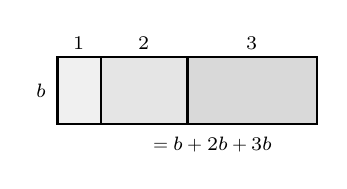
\begin{tikzpicture}[x=1cm, y=1cm, every node/.style={font=\scriptsize, text=black}]
      \draw[black, line width=0.8pt, fill=gray!12] (0.4,0.2) rectangle (0.95,1.05);
      \draw[black, line width=0.8pt, fill=gray!20] (0.95,0.2) rectangle (2.05,1.05);
      \draw[black, line width=0.8pt, fill=gray!30] (2.05,0.2) rectangle (3.70,1.05);
      \node at (0.20,0.62) {$b$};
      \node at (0.675,1.22) {$1$};
      \node at (1.50,1.22) {$2$};
      \node at (2.875,1.22) {$3$};
      \node at (2.05,-0.06) {ផ្ទៃសរុប $= b + 2b + 3b$};
    \end{tikzpicture}
  \end{minipage}\hfill
  \begin{minipage}[c]{13.2cm}
    $\bullet$ \textbf{១) ផលបូកផ្ទៃក្រឡា (ទំ.៥៣)៖} $b + 2b + 3b = (1 + 2 + 3)b =$ \ansbox[2.0cm]\\[3pt]
    $\bullet$ \textbf{២) ផលដកឯកធា (ទំ.៥៣)៖} $5x - 2x = (5 - 2)x =$ \ansbox[2.0cm]\\[3pt]
    $\bullet$ \textbf{៣) លំហាត់គំរូ (ទំ.៥៤ ក, ខ)៖} ក) $2xy + 5xy = (2+5)xy =$ \ansbox[2.2cm]\\[3pt]
    \hspace*{0.3cm}ខ) $3ab^2 + 7ab^2 + ab^2 = (3 + 7 + \dotline[0.8cm])ab^2 =$ \ansbox[2.2cm]
  \end{minipage}
\end{tcolorbox}

\vspace{4pt}
\textbf{សកម្មភាព ២ (\en{E2-B} — ៦ នាទី)៖ វិធីគុណឯកធា និងវិធីចែកឯកធា (ទំ.៥៤--៥៥)}

\begin{tcolorbox}[
  enhanced, sharp corners, colback=white, colframe=black,
  boxrule=0.8pt, boxsep=2.5pt, top=4pt, bottom=4pt, left=6pt, right=6pt
]
  $\bullet$ \textbf{១) សួនច្បារចតុកោណកែងបណ្ដោយ $5x$ និងទទឹង $2x$ (ទំ.៥៤)៖} ផ្ទៃក្រឡា $(5x)(2x) = (5)(2)(x)(x) =$ \ansbox[2.2cm]\\[3pt]
  $\bullet$ \textbf{២) គុណឯកធា (ឧ.២ ទំ.៥៤)៖} $(4x^2yc^4)(3xy^3c) = (4)(3)x^{2+1}y^{1+3}c^{4+1} =$ \ansbox[2.8cm]\\[3pt]
  $\bullet$ \textbf{៣) ស្រះទឹកផ្ទៃក្រឡា $16xy^2$ និងទទឹង $4y$ (ទំ.៥៥)៖} បណ្ដោយ $= \dfrac{16xy^2}{4y} =$ \ansbox[2.2cm]\\[3pt]
  $\bullet$ \textbf{៤) ចែកឯកធា (ឧ.២ ទំ.៥៥)៖} $(8x^4y^5) \div (16x^2y^3) = \dfrac{8}{16}x^{4-2}y^{5-3} =$ \ansbox[2.6cm]
\end{tcolorbox}

\vfill

% --- E3 Explain ---
\secstrip{ផ្នែកទី ៣ \enbf{(E3 - Explain)} ៖ ក្បួនគោលទាំង ៣ និងធនាគារហេតុផល \enbf{B\&W}}{រយៈពេល ៦ នាទី}

\begin{tcolorbox}[
  enhanced, sharp corners, colback=white, colframe=black,
  boxrule=0.85pt, boxsep=2.5pt, top=4pt, bottom=4pt, left=6pt, right=6pt
]
  $\bullet$ \textbf{១) បូក/ដកឯកធាដូចគ្នា៖} បូកឬដកតែផ្នែក \dotline[2.2cm] រួចគុណនឹងផ្នែក \dotline[2.4cm] ដដែល ។\\[3pt]
  $\bullet$ \textbf{២) គុណឯកធា៖} គុណមេគុណនឹងមេគុណ ហើយ\textbf{បូក}និទស្សន្ត ($x^m \cdot x^n = x^{\dotline[1.0cm]}$); \quad
  \textbf{៣) ចែកឯកធា៖} ចែកមេគុណ ហើយ\textbf{ដក}និទស្សន្ត ($x^m \div x^n = x^{\dotline[1.0cm]}$) ។\\[4pt]
  \tikz\draw[black, dashed, line width=0.5pt] (0,0) -- (18.4cm,0);\\[3pt]
  \fontsize{8.8pt}{13.0pt}\selectfont
  \textbf{ធនាគារហេតុផល (\en{Warrant Bank})៖} \quad
  \cnum{1} បូក/ដកឯកធាដូចគ្នា៖ រក្សាផ្នែកអថេរដដែល \quad
  \cnum{2} មេគុណលាក់មុខ៖ $ab^2 = 1ab^2$\\
  \cnum{3} គុណឯកធា៖ គុណមេគុណ បូកនិទស្សន្ត \quad
  \cnum{4} ចែកឯកធា៖ សម្រួលប្រភាគមេគុណ ដកនិទស្សន្ត
\end{tcolorbox}

% ============================================================================
% ទំព័រទី ២៖ សន្លឹកកិច្ចការសិស្ស (ផ្នែកខាងខ្នង៖ E4 -> E5 -> កិច្ចការផ្ទះ)
% ============================================================================
\clearpage
\pagebanner{សន្លឹកកិច្ចការសិស្ស \enbf{(}៥\enbf{.}១\enbf{.}៤\enbf{--}៥\enbf{.}១\enbf{.}៦ ប្រមាណវិធីលើឯកធា\enbf{)} \enbf{--} ផ្នែកខាងខ្នង}{ថ្នាក់ទី៨ \en{|} សៀវភៅគោល ទំ.៥៤--៥៦, ៧២}

% --- E4 Elaborate ---
\secstrip{ផ្នែកទី ៤ \enbf{(E4 - Elaborate)} ៖ លំហាត់គំរូទាំង ៣ ផ្នែក និងប្លង់ភូមិគ្រឹះ (ទំ.៥៤--៥៦)}{រយៈពេល ១០ នាទី}

\begin{tcolorbox}[
  enhanced, sharp corners, colback=white, colframe=black,
  boxrule=0.8pt, boxsep=2.5pt, top=4pt, bottom=4pt, left=6pt, right=6pt
]
  \textbf{១) លំហាត់គំរូបូកនិងដកឯកធាដូចគ្នា (ទំ.៥៤ គ, ឃ)៖}\\[3pt]
  \hspace*{0.3cm}$\bullet$ គ) $8x^2y^3z - 3x^2y^3z - 7x^2y^3z = (8 - 3 - 7)x^2y^3z =$ \ansbox[2.8cm]\\[3pt]
  \hspace*{0.3cm}$\bullet$ ឃ) $10x^2y + x^2y - 5x^2y = (10 + \dotline[0.8cm] - 5)x^2y =$ \ansbox[2.6cm]\\[4pt]
  \textbf{២) លំហាត់គំរូផ្ទៃក្រឡាប្លង់ភូមិគ្រឹះ (ទំ.៥៥ — បណ្ដោយ $18a$ និងទទឹង $12a$)៖}\\[3pt]
  \hspace*{0.3cm}$A = (18a)(12a) = (18)(12)(a)(a) =$ \ansbox[2.6cm] ឯកតាផ្ទៃ ។\\[4pt]
  \textbf{៣) លំហាត់គំរូវិធីចែកឯកធា (ទំ.៥៦ ក, ខ, គ)៖}\\[3pt]
  \hspace*{0.3cm}ក) $(5xy^3)\div(xy) =$ \ansbox[2.0cm] \quad
  ខ) $\dfrac{18xyz^3}{9yz^2} =$ \ansbox[2.0cm] \quad
  គ) $1a^2b^3 \div 2ab =$ \ansbox[2.2cm]\\[3pt]
  \fontsize{8.8pt}{13.0pt}\selectfont
  \textbf{ឆ្លុះបញ្ចាំង (\en{EIA Looking-Back})៖} ហេតុអ្វី $1a^2b^3 \div 2ab$ មានមេគុណស្មើ $\dfrac{1}{2}$ មិនមែនស្មើ $2$? \textbf{ព្រោះ} \dotline[5.2cm] ។
\end{tcolorbox}

\vspace{4pt}

% --- E5 Evaluate ---
\secstrip{ផ្នែកទី ៥ \enbf{(E5 - Evaluate)} ៖ ប្រតិបត្តិ (ទំ.៥៤--៥៦) សំណួរវិនិច្ឆ័យ \enbf{A--D} និងសំបុត្រចេញ}{រយៈពេល ១០ នាទី}

\begin{tcolorbox}[
  enhanced, sharp corners, colback=white, colframe=black,
  boxrule=0.8pt, boxsep=2.5pt, top=4pt, bottom=4pt, left=6pt, right=6pt
]
  \textbf{១) លំហាត់ប្រតិបត្តិចម្រុះ (ទំ.៥៤--៥៦) — គណនាជាក្រុម ៣ នាក់៖}\\[3pt]
  \hspace*{0.3cm}$\bullet$ បូកដក (ទំ.៥៤ ក, គ)៖ \quad $5x^2y - 3x^2y =$ \ansbox[2.4cm] \qquad $ax^2y^2 + 3ax^2y^2 =$ \ansbox[2.6cm]\\[4pt]
  \hspace*{0.3cm}$\bullet$ គុណនិងចែក (ទំ.៥៥ ក, ទំ.៥៦ ឃ)៖ \quad $(5xy^3)(x^2y) =$ \ansbox[2.4cm] \qquad $\dfrac{xyz^3}{yz^2} =$ \ansbox[2.4cm]\\[4pt]
  \textbf{២) បិទបេសកកម្ម \en{E1}៖} សិស្ស \dotline[1.0cm] ត្រឹមត្រូវ ព្រោះ $5x^2 + 3x^2 =$ \ansbox[2.0cm] (ឯ $(5x^2)(3x^2) =$ \dotline[1.8cm]) ។
\end{tcolorbox}

\vspace{4pt}

\begin{tcolorbox}[
  enhanced, sharp corners, colback=white, colframe=black,
  boxrule=0.8pt, boxsep=2.5pt, top=4pt, bottom=4pt, left=6pt, right=6pt
]
  \textbf{៣) សំណួរវិនិច្ឆ័យ \en{A--D} (គណនាផលគុណឯកធា $(-4a^2b^3)(3ab^2)$ — គូសរង្វង់ រួចលើកម្រាមដៃ ១--៤)៖}\\[3pt]
  \textbf{\en{A.}} $-a^3b^5$ \qquad\qquad
  \textbf{\en{B.}} $-12a^2b^6$ \qquad\qquad
  \textbf{\en{C.}} $-12a^3b^5$ \qquad\qquad
  \textbf{\en{D.}} $12a^3b^5$\\[4pt]
  \tikz\draw[black, dashed, line width=0.5pt] (0,0) -- (18.4cm,0);\\[3pt]
  \textbf{៤) សំបុត្រចេញ ៦០ វិនាទី៖} គណនា៖ \quad ក) $7m^2n - m^2n =$ \ansbox[2.4cm] \qquad ខ) $\dfrac{12x^5y^2}{4x^2y} =$ \ansbox[2.4cm]
\end{tcolorbox}

\vfill

% --- Homework ---
\begin{tcolorbox}[
  enhanced, sharp corners, colback=panelgray, colframe=black,
  boxrule=0.95pt, boxsep=2pt, top=3.5pt, bottom=3.5pt, left=6pt, right=6pt
]
  {\muol\fontsize{9.0pt}{13.0pt}\selectfont កិច្ចការផ្ទះ \enbf{(}សៀវភៅគោល ទំ.៥៤--៥៦ និង ទំ.៧២ លេខ ៣ ក\enbf{)}}\\[2.5pt]
  \fontsize{8.8pt}{13.0pt}\selectfont
  $\bullet$ \textbf{១) បូកដក៖} ទំ.៥៤ (ច) $\dfrac{1}{2}ac^2b^3 + \left(-\dfrac{1}{2}ac^2b^3\right) + 7ac^2b^3$ និង ទំ.៧២ \#3 ក) $3x^2 + 7x^2 - 5x^2$ ។\\
  $\bullet$ \textbf{២) គុណចែក៖} ទំ.៥៥ (គ) $\left(\dfrac{1}{2}ab^3\right)(3a^2b^2)$, \ ទំ.៥៦ (ង) $\dfrac{ax^7b^5}{ax^5b^3}$ និង (ច) $81z^{12}b^3 \div 3z^{12}b$ ។ \textbf{អានមុន៖} ២.១--២.៣ (ទំ.៥៦--៥៩) ។
\end{tcolorbox}

% ============================================================================
% ទំព័រទី ៣៖ ទំព័រគ្រូបង្រៀន (គំរូប្លង់ក្ដារខៀន ៣ ផ្នែក + ចម្លើយផ្ទៀងផ្ទាត់រហ័ស)
% ============================================================================
\clearpage
\pagebanner{ទំព័រគ្រូបង្រៀន ៖ ប្លង់ក្ដារខៀន \enbf{(}គ្មាន \enbf{LCD)} និងចម្លើយផ្ទៀងផ្ទាត់រហ័ស}{៥.១.៤--៥.១.៦ ប្រមាណវិធីលើឯកធា (\en{ALG52})}

\secstrip{១. គំរូប្លង់បែងចែកក្ដារខៀន ៣ ផ្នែក សម្រាប់ថ្នាក់រៀនគ្មាន \enbf{LCD}}{សម្រាប់គ្រូប្រើដីស/ហ្វឺត}

\begin{center}
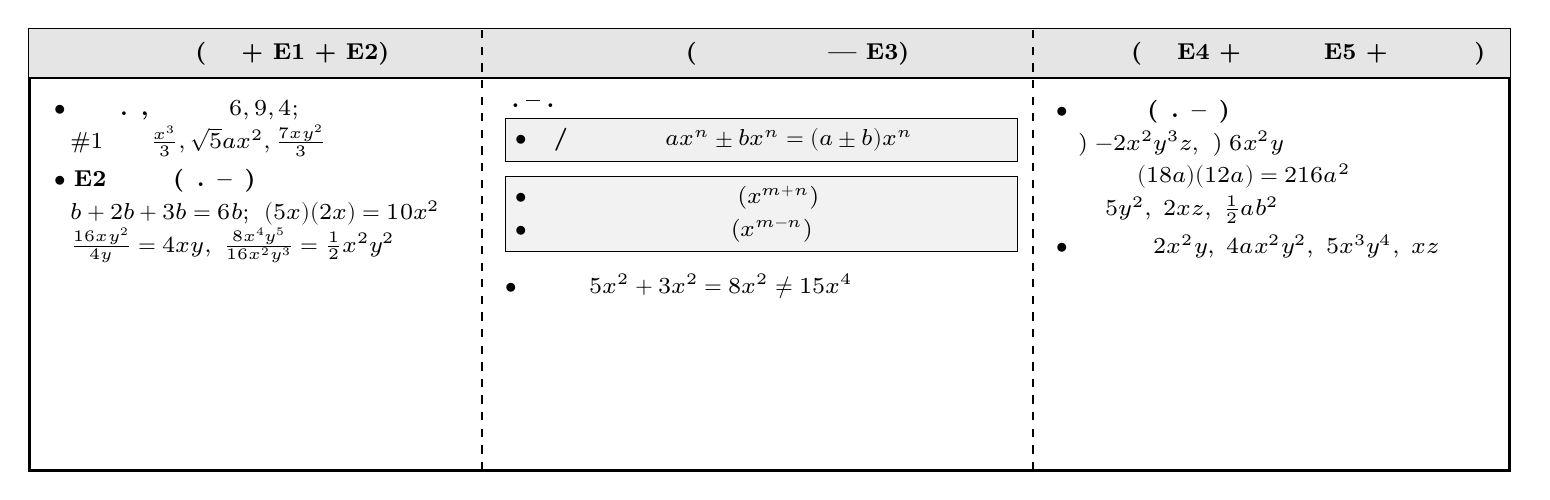
\begin{tikzpicture}[x=1cm, y=1cm, every node/.style={font=\fontsize{8.3pt}{11.8pt}\selectfont, text=black}]
  \draw[black, line width=1.1pt] (0,0) rectangle (18.8,5.60);
  \fill[gray!20] (0,4.98) rectangle (18.8,5.60);
  \draw[black, line width=0.7pt] (0,4.98) -- (18.8,4.98);
  \draw[black, dashed, line width=0.7pt] (5.75,0) -- (5.75,5.60);
  \draw[black, dashed, line width=0.7pt] (12.75,0) -- (12.75,5.60);

  \node at (2.875,5.29) {\textbf{ផ្នែកឆ្វេង (កំណែ + \en{E1} + \en{E2})}};
  \node at (9.25,5.29) {\textbf{ផ្នែកកណ្ដាល (ខ្លឹមសារគោលរក្សាទុក — \en{E3})}};
  \node at (15.775,5.29) {\textbf{ផ្នែកស្ដាំ (គំរូ \en{E4} + ប្រតិបត្តិ \en{E5} + កិច្ចការផ្ទះ)}};

  % Left
  \node[anchor=north west, text width=5.35cm] at (0.20,4.82) {%
    $\bullet$ \textbf{កំណែ ទំ.៥៣, ៧២៖} ដឺក្រេ $6, 9, 4$;\\
    \hspace*{0.2cm}\#1 ឯកធា៖ $\tfrac{x^3}{3}, \sqrt{5}ax^2, \tfrac{7xy^2}{3}$\\[2pt]
    $\bullet$ \textbf{\en{E2} គំរូផ្ទៃ (ទំ.៥៣--៥៥)៖}\\
    \hspace*{0.2cm}$b+2b+3b = 6b$; \ $(5x)(2x) = 10x^2$\\
    \hspace*{0.2cm}$\tfrac{16xy^2}{4y} = 4xy, \ \tfrac{8x^4y^5}{16x^2y^3} = \tfrac{1}{2}x^2y^2$
  };

  % Center
  \node[anchor=north west, text width=6.65cm] at (5.92,4.82) {%
    {\muol\fontsize{8.5pt}{12pt}\selectfont ១\enbf{.}៤\enbf{--}១\enbf{.}៦ ប្រមាណវិធីលើឯកធា}\\[3pt]
    \tikz\node[draw=black, fill=gray!12, inner sep=3.5pt, text width=6.25cm]{%
      $\bullet$ \textbf{បូក/ដកឯកធាដូចគ្នា៖} $ax^n \pm bx^n = (a\pm b)x^n$
    };\\[4pt]
    \tikz\node[draw=black, fill=gray!10, inner sep=3.5pt, text width=6.25cm]{%
      $\bullet$ \textbf{គុណឯកធា៖} គុណមេគុណ បូកនិទស្សន្ត ($x^{m+n}$)\\
      $\bullet$ \textbf{ចែកឯកធា៖} ចែកមេគុណ ដកនិទស្សន្ត ($x^{m-n}$)
    };\\[3pt]
    $\bullet$ ប្រៀបធៀប៖ $5x^2+3x^2=8x^2 \neq 15x^4$
  };

  % Right
  \node[anchor=north west, text width=5.8cm] at (12.92,4.82) {%
    $\bullet$ \textbf{លំហាត់គំរូ (ទំ.៥៤--៥៦)៖}\\
    \hspace*{0.2cm}គ) $-2x^2y^3z$, ឃ) $6x^2y$\\
    \hspace*{0.2cm}ភូមិគ្រឹះ $(18a)(12a) = 216a^2$\\
    \hspace*{0.2cm}ចែក៖ $5y^2, \ 2xz, \ \tfrac{1}{2}ab^2$\\[2pt]
    $\bullet$ \textbf{ប្រតិបត្តិ៖} $2x^2y, \ 4ax^2y^2, \ 5x^3y^4, \ xz$
  };
\end{tikzpicture}
\end{center}

\vspace{4pt}
\secstrip{២. ចម្លើយផ្ទៀងផ្ទាត់រហ័សសម្រាប់សន្លឹកកិច្ចការសិស្ស \enbf{(}ទំព័រ ១ និង ទំព័រ ២\enbf{)}}{\en{Answer Key}}

\begin{tcolorbox}[
  enhanced, sharp corners, colback=white, colframe=black,
  boxrule=0.8pt, boxsep=2pt, top=4pt, bottom=4pt, left=6pt, right=6pt
]
  \fontsize{9.0pt}{13.5pt}\selectfont
  $\bullet$ \textbf{ផ្នែក \en{E1}៖} \textbf{សិស្ស ខ} ត្រឹមត្រូវ ($5x^2+3x^2 = 8x^2$) ព្រោះបូកការេផ្ទៃ $x^2$ បាន $8$ បន្ទះនៃ $x^2$ ។\\[2pt]
  $\bullet$ \textbf{ផ្នែក \en{E2}៖} \textbf{សកម្មភាព ១៖} $6b, \ 3x, \ 7xy$ និង $(3+7+1)ab^2 = 11ab^2$ ។ \textbf{សកម្មភាព ២៖} $10x^2, \ 12x^3y^4c^5, \ 4xy, \ \frac{1}{2}x^2y^2$ ។\\[2pt]
  $\bullet$ \textbf{ផ្នែក \en{E4}៖} ១) គ) $-2x^2y^3z$, ឃ) $(10+1-5)x^2y = 6x^2y$; ២) $216a^2$; ៣) ក) $5y^2$, ខ) $2xz$, គ) $\frac{1}{2}ab^2$ ។\\[2pt]
  $\bullet$ \textbf{ផ្នែក \en{E5}៖} ១) $2x^2y, \ 4ax^2y^2, \ 5x^3y^4, \ xz$; ២) សិស្ស ខ ($8x^2$ ឯគុណបាន $15x^4$); ៣) \textbf{ជម្រើស \en{C}} ($-12a^3b^5$); ៤) ក) $6m^2n$, ខ) $3x^3y$ ។
\end{tcolorbox}

\vspace{4pt}
\secstrip{៣. ចម្លើយលម្អិតនៃកិច្ចការផ្ទះ \enbf{(}សម្រាប់ផ្ទៀងនៅដើមម៉ោងបន្ទាប់ ៥\enbf{.}២\enbf{.}១\enbf{)}}{សៀវភៅគោល ទំ.៥៤--៥៦, ៧២}

\begin{tcolorbox}[
  enhanced, sharp corners, colback=white, colframe=black,
  boxrule=0.8pt, boxsep=2pt, top=4pt, bottom=4pt, left=6pt, right=6pt
]
  \fontsize{8.8pt}{13.2pt}\selectfont
  $\bullet$ \textbf{១) បូកដក៖} ទំ.៥៤ (ច) $\left(\frac{1}{2} - \frac{1}{2} + 7\right)ac^2b^3 = \mathbf{7ac^2b^3}$; \quad ទំ.៧២ \#3 ក) $3x^2+7x^2-5x^2 = (3+7-5)x^2 = \mathbf{5x^2}$ ។\\[2pt]
  $\bullet$ \textbf{២) គុណចែក៖} ទំ.៥៥ (គ) $\left(\frac{1}{2}ab^3\right)(3a^2b^2) = \mathbf{\dfrac{3}{2}a^3b^5}$; \quad ទំ.៥៦ (ង) $\dfrac{ax^7b^5}{ax^5b^3} = \mathbf{x^2b^2}$; \quad ទំ.៥៦ (ច) $81z^{12}b^3 \div 3z^{12}b = 27z^{12-12}b^{3-1} = \mathbf{27b^2}$ ។
\end{tcolorbox}

\end{document}
